\documentclass[11pt,a4paper]{article}
\usepackage[utf8]{inputenc}
\usepackage[T1]{fontenc}
\usepackage{amsmath,amssymb,amsfonts}
\usepackage{geometry}
\geometry{a4paper, margin=0.86in, headheight=26pt, headsep=12pt}
\usepackage{lmodern}
\usepackage{xcolor}

% Custom Color Palette
\definecolor{primaryblue}{RGB}{13, 71, 161}    % Deep Blue #0D47A1
\definecolor{secondaryblue}{RGB}{25, 118, 210} % Medium Blue #1976D2
\definecolor{accentred}{RGB}{198, 40, 40}     % Dark Red #C62828
\definecolor{accentgreen}{RGB}{46, 125, 50}    % Dark Green #2E7D32
\definecolor{bglight}{RGB}{248, 249, 250}     % Soft Gray background
\definecolor{bordergrey}{RGB}{207, 216, 220}  % Slate border
\definecolor{darkslate}{RGB}{38, 50, 56}      % Dark slate text
\definecolor{goldyellow}{RGB}{230, 140, 0}    % Deep Gold

\usepackage{tcolorbox}

% Custom tcolorbox Callout Boxes (Standard base tcolorbox for full compatibility)
\newtcolorbox{defbox}[1][Definition]{%
  colback=primaryblue!6!white,
  colframe=primaryblue,
  fonttitle=\bfseries\color{white},
  title={Resource Planning Definition: #1},
  arc=4pt,
  boxrule=1.5pt,
  before skip=10pt,
  after skip=10pt
}

\newtcolorbox{keybox}[1][Key Concept]{%
  colback=accentred!6!white,
  colframe=accentred,
  fonttitle=\bfseries\color{white},
  title={Key Theoretical Concept: #1},
  arc=4pt,
  boxrule=1.5pt,
  before skip=10pt,
  after skip=10pt
}

\newtcolorbox{modelbox}[1][Geographic Model]{%
  colback=secondaryblue!6!white,
  colframe=secondaryblue,
  fonttitle=\bfseries\color{white},
  title={Planning Model / Policy Framework: #1},
  arc=4pt,
  boxrule=1.5pt,
  before skip=10pt,
  after skip=10pt
}

\newtcolorbox{casebox}[1][Case Study]{%
  colback=accentgreen!6!white,
  colframe=accentgreen,
  fonttitle=\bfseries\color{white},
  title={Regional Case Study: #1},
  arc=4pt,
  boxrule=1.5pt,
  before skip=10pt,
  after skip=10pt
}

\newtcolorbox{exambox}[1][Exam Focus]{%
  colback=goldyellow!8!white,
  colframe=goldyellow!95!black,
  fonttitle=\bfseries\color{white},
  title={Exam Focus \& Model Answer Outline: #1},
  arc=4pt,
  boxrule=1.5pt,
  before skip=10pt,
  after skip=10pt
}

\usepackage{tikz}
\usetikzlibrary{arrows.meta, positioning, calc, shapes, patterns}

\usepackage{fancyhdr}
\pagestyle{fancy}
\fancyhf{}
\fancyhead[L]{\parbox[b]{0.65\textwidth}{\raggedright\small\color{darkslate}\bfseries GGRMN41: Resource Planning}}
\fancyhead[R]{\small\color{primaryblue}\bfseries Theory Course | sciqb.com}
\fancyfoot[L]{\sffamily\color{gray}\small Notes by Aryan Maurya (sciqb.com)}
\fancyfoot[C]{\thepage}
\fancyfoot[R]{\sffamily\color{secondaryblue}\small\bfseries\href{https://sciqb.com}{sciqb.com}}
\renewcommand{\headrulewidth}{0.6pt}

\fancypagestyle{plain}{%
  \fancyhf{}%
  \fancyfoot[L]{\sffamily\color{gray}\small Notes by Aryan Maurya (sciqb.com)}%
  \fancyfoot[C]{\thepage}%
  \fancyfoot[R]{\sffamily\color{secondaryblue}\small\bfseries\href{https://sciqb.com}{sciqb.com}}%
  \renewcommand{\headrulewidth}{0pt}%
}

\usepackage{hyperref}
\hypersetup{
    colorlinks=true,
    linkcolor=secondaryblue,
    citecolor=accentred,
    urlcolor=primaryblue,
    pdftitle={GGRMN41 Resource Planning Master Exam Notes},
    pdfauthor={Aryan Maurya (sciqb.com)}
}

\usepackage{microtype}
\usepackage{enumitem}
\usepackage{booktabs}
\usepackage{tabularx}
\usepackage{titlesec}

\titleformat{\section}{\Large\bfseries\color{primaryblue}}{\thesection}{1em}{}[\titlerule]
\titleformat{\subsection}{\large\bfseries\color{secondaryblue}}{\thesubsection}{1em}{}
\titleformat{\subsubsection}{\bfseries\color{darkslate}}{\thesubsubsection}{1em}{}

\begin{document}

% Title Banner
\begin{center}
  \tcbset{colback=primaryblue,colframe=primaryblue,arc=6pt}
  \begin{tcolorbox}[width=\textwidth,coltext=white,halign=center]
    \vspace{4pt}
    {\Huge \bfseries RESOURCE PLANNING}\\[6pt]
    {\Large \bfseries Course Code: GGRMN41 \quad|\quad Credits: 3 (Theory)}\\[4pt]
    {\small Department of Geography \quad\textbullet\quad Course Type: Theory \quad\textbullet\quad Master Study Guide}
    \vspace{4pt}
  \end{tcolorbox}
  \vspace{6pt}
  {\Large \bfseries Comprehensive Master Exam Notes \& Reference Textbook}\\[2pt]
  {\small Prepared by Aryan Maurya for Academic Excellence \& University Examinations \quad|\quad \textbf{sciqb.com}}
\end{center}

\vspace{8pt}
\tableofcontents
\newpage

% ==========================================
% UNIT I: BASIC FRAMEWORK OF RESOURCE PLANNING
% ==========================================
\section{Unit I: Basic Framework of Resource Planning}

\subsection{Nature, Scope, and Relevance of Resource Geography}

\begin{defbox}[Resource Geography]
Resource Geography is a vital sub-discipline of economic geography that investigates the spatial distribution, physical appraisal, socio-economic utilization, conservation, and institutional planning of natural and human resources across the earth's surface over time.
\end{defbox}

\subsubsection{Scope and Academic Relevance}
\begin{itemize}[leftmargin=*]
  \item \textbf{Interface with Sister Disciplines}: Resource geography lies at the intersection of Physical Geography (geomorphology, hydrology, soil science, climatology), Economics (resource allocation, cost-benefit analysis), Environmental Science (ecology, sustainability), and Spatial Planning.
  \item \textbf{Core Objectives}:
  \begin{enumerate}
    \item Mapping and surveying the spatial pattern of natural and human resource endowments.
    \item Analyzing the physical and technological mechanisms of resource transformation.
    \item Evaluating the environmental impacts of resource exploitation.
    \item Formulating spatial planning strategies for sustainable resource management and regional development.
  \end{enumerate}
\end{itemize}

\subsubsection{Erich Zimmermann's Dynamic Resource Paradigm}
The theoretical foundation of modern Resource Geography is anchored in \textbf{Erich W. Zimmermann's} functional concept (\textit{World Resources and Industries}, 1933, 1951):
\begin{quote}
  ``Resources are not, they become; they are not static gifts of nature, but expand and shrink in response to human wants and human abilities.''
\end{quote}

\begin{itemize}[leftmargin=*]
  \item \textbf{Neutral Stuff}: Substances in nature exist initially as ``neutral stuff'' (e.g., crude petroleum before internal combustion engines, bauxite before electrolytic smelting, solar radiation prior to photovoltaic technology).
  \item \textbf{Functional Triplet}: Neutral stuff is transformed into a functional \textbf{resource} through the interaction of three core variables:
  \begin{enumerate}
    \item \textbf{Man} (the active agent possessing physical needs, intellectual desires, and labor power).
    \item \textbf{Nature} (the physical environment providing matter, energy, and spatial medium).
    \item \textbf{Culture} (the accumulated body of scientific knowledge, technological tools, capital infrastructure, and legal/social institutions).
  \end{enumerate}
  \item \textbf{Resistances}: Environmental hazards, rugged terrain, extreme climates, technological backwardness, capital scarcity, and socio-political conflicts act as \textbf{resistances} that counteract resource creation.
\end{itemize}

\subsubsection{Gottfried Pfeifer \& Zimmermann's Resource Typology}
Resources are categorized according to their spatial frequency of occurrence:
\begin{enumerate}[leftmargin=*]
  \item \textbf{Ubiquities}: Available everywhere across the globe (e.g., atmospheric nitrogen, oxygen, sunlight).
  \item \textbf{Commonalities}: Found in many parts of the world (e.g., arable soil, fresh water, forest timber).
  \item \textbf{Rarities}: Found in only a few specific geographic locations (e.g., tin, gold, platinum, petroleum deposits).
  \item \textbf{Uniquities}: Occurring in only one specific locality on earth (e.g., natural cryolite historically found only in Ivittuut, Greenland).
\end{enumerate}

\subsubsection{Multidimensional Classification of Resources}
\begin{table}[h!]
\centering
\small
\begin{tabularx}{\textwidth}{l X X}
\toprule
\textbf{Classification Basis} & \textbf{Resource Category} & \textbf{Core Characteristics \& Examples} \\
\midrule
\textbf{By Origin} & Biotic & Organic origin; living organisms, forests, crops, coal, crude oil \\
 & Abiotic & Inorganic origin; rocks, minerals, soils, land, water, air \\
\midrule
\textbf{By Exhaustibility} & Renewable / Flow & Naturally replenished over time; solar, wind, hydro, forests \\
 & Non-Renewable / Stock & Finite stock created over geological time; coal, iron ore, petroleum \\
\midrule
\textbf{By Development Status} & Potential & Quantity known, but unexploited due to technology/capital gap \\
 & Developed / Actual & Surveyed, quantified, and actively extracted with current technology \\
 & Stock & Possesses energy potential, but lacks extraction technology \\
 & Reserve & Subset of developed resources saved for future emergency use \\
\midrule
\textbf{By Ownership} & Individual & Privately owned property, land plots, personal wells \\
 & Community & Shared public assets; pasture lands, village ponds, burial grounds \\
 & National & Assets within national boundaries and Exclusive Economic Zone (EEZ) \\
 & International / Global & Global Commons (high seas $>200$ nautical miles, Antarctica, outer space) \\
\bottomrule
\end{tabularx}
\caption{Comprehensive Classification Matrix of World Resources}
\end{table}

\subsubsection{Resource Planning: Concept, Need, Objectives, and Stages}

\begin{defbox}[Resource Planning]
Resource Planning is the scientific, rational, systematic, and balanced strategy for the identification, appraisal, allocation, conservation, and sustainable utilization of natural and human resources across space and time to achieve optimal socio-economic development without causing environmental degradation.
\end{defbox}

\begin{itemize}[leftmargin=*]
  \item \textbf{Need for Resource Planning in Developing Countries (Special Reference to India)}:
  \begin{enumerate}
    \item \textit{Extreme Spatial Imbalance}: India exhibits acute regional disparities in resource endowment. The Chota Nagpur Plateau is rich in coal and minerals but socio-economically backward. Arunachal Pradesh has immense hydro potential ($>30\%$) but lacks infrastructure. Rajasthan possesses vast solar/wind potential but acute water scarcity.
    \item \textit{Population Pressure}: High population density puts immense pressure on finite arable land and groundwater tables.
    \item \textit{Ecological Protection}: Prevents reckless extraction leading to deforestation, topsoil erosion, and toxic pollution.
  \end{enumerate}

  \item \textbf{Four Institutional Stages of Resource Planning}:
  \begin{enumerate}
    \item \textbf{Identification and Inventory}: Conducting ground surveys, aerial photography, satellite mapping, and compiling comprehensive resource registers.
    \item \textbf{Quantitative \& Qualitative Appraisal}: Evaluating total reserves, mineral grade, economic cost of extraction, and environmental feasibility.
    \item \textbf{Formulation of Resource Development Plan}: Designing technological blueprints, infrastructure investments, and aligning resource plans with national planning goals (NITI Aayog vision).
    \item \textbf{Implementation \& Periodic Monitoring}: Allocating institutional roles, executing ground operations, and evaluating ecological feedback loops.
  \end{enumerate}
\end{itemize}

\subsection{Methods and Techniques of Resource Appraisal}

\begin{defbox}[Resource Appraisal]
Resource Appraisal is the multi-disciplinary methodology of measuring, mapping, evaluating, and analyzing the physical quantity, quality, economic viability, technological feasibility, and environmental consequences of resource exploitation.
\end{defbox}

\subsubsection{1. Survey and Geospatial Technology Techniques}
\begin{itemize}[leftmargin=*]
  \item \textbf{Ground Surveys \& Geological Coring}: Traditional field sampling, strike-and-dip geological measurements, soil profile coring, and stream gauging.
  \item \textbf{Remote Sensing (RS)}: Satellite sensors (ISRO IRS series, Cartosat, Resourcesat, Landsat, Sentinel) capture electromagnetic radiation reflected from Earth's surface.
  \begin{itemize}
    \item \textit{Multi-spectral \& Hyperspectral Imaging}: Enables rapid identification of mineral deposits, forest canopy density, and soil moisture levels.
    \item \textit{Normalized Difference Vegetation Index (NDVI)}: Measures green biomass density and crop health:
    \begin{equation}
      \text{NDVI} = \frac{\text{NIR} - \text{Red}}{\text{NIR} + \text{Red}}
    \end{equation}
    Where NIR is Near-Infrared reflectance and Red is Visible Red reflectance. Range spans from $-1.0$ (water) to $+1.0$ (dense forest).
  \end{itemize}
  \item \textbf{Geographic Information Systems (GIS)}: Spatial overlay analysis, 3D Digital Elevation Model (DEM) generation, watershed boundary delineation, and multi-criteria land-suitability evaluation.
\end{itemize}

\subsubsection{2. Economic Appraisal Techniques}
Economic appraisal evaluates the monetized financial return and social viability over project lifecycles:

\begin{enumerate}[leftmargin=*]
  \item \textbf{Cost-Benefit Analysis (CBA)}: Quantifies all direct and indirect social costs versus social benefits. A project is justified if the Benefit-Cost Ratio ($\text{BCR} = \frac{\text{Total Discounted Benefits}}{\text{Total Discounted Costs}}) > 1.0$.
  
  \item \textbf{Net Present Value (NPV)}: Discounts future cash/environmental flows to present value using a discount rate $r$:
  \begin{equation}
    \text{NPV} = \sum_{t=0}^{n} \frac{B_t - C_t}{(1 + r)^t}
  \end{equation}
  Where $B_t$ is annual benefit, $C_t$ is annual cost, $r$ is discount rate, $n$ is project lifespan. If $\text{NPV} > 0$, investment is economically sound.

  \item \textbf{Internal Rate of Return (IRR)}: The specific discount rate $r^*$ at which $\text{NPV} = 0$. If IRR exceeds market interest rates, the project is financially viable.
\end{enumerate}

\subsubsection{3. Ecological and Environmental Appraisal Techniques}
\begin{enumerate}[leftmargin=*]
  \item \textbf{Environmental Impact Assessment (EIA)}: A statutory process evaluating potential environmental degradation (air, water, noise, biodiversity loss) before project approval.
  \item \textbf{Ecological Footprint Analysis}: Formulated by William Rees and Mathis Wackernagel. Measures the biologically productive land and water area required to supply the resources consumed and absorb the wastes generated by a human population (measured in \textbf{global hectares per capita}).
  \item \textbf{Carrying Capacity Analysis}: Evaluates the maximum human population or economic activity that an ecosystem can sustain indefinitely without irreversible ecological degradation.
  \item \textbf{Ecosystem Services Valuation (ESV)}: Championed by Robert Costanza et al. (1997). Quantifies the global economic value of 17 ecosystem services (e.g., nutrient cycling, climate regulation, pollination, waste treatment) estimated at over \$33 trillion annually.
  \item \textbf{System of Environmental-Economic Accounting (SEEA)}: UN framework integrating natural capital accounting into standard national GDP accounts.
\end{enumerate}

\subsection{Seven Major Approaches in Resource Geography \& Management}

\begin{modelbox}[Seven Approaches in Resource Geography]
Resource management has evolved through seven distinct theoretical perspectives (Gautam 2011; UGC Module RG-07) that guide spatial research and policy formulation.
\end{modelbox}

\begin{table}[h!]
\centering
\small
\begin{tabularx}{\textwidth}{l X X X}
\toprule
\textbf{Approach} & \textbf{Theoretical Foundation} & \textbf{Core Focus \& Methodology} & \textbf{Policy / Practical Application} \\
\midrule
\textbf{1. Ecological} & Ecosystem science (E. Odum); physical sciences & Interconnectedness of biotic/abiotic systems; energy flow efficiency; natural carrying capacity & Ecosystem management, biodiversity conservation, EIA \\
\midrule
\textbf{2. Economic} & Neo-classical economics; resource allocation & Market pricing, supply-demand equilibrium, profit maximization, Hotelling extraction rate & Carbon credit trading, water pricing, resource taxation \\
\midrule
\textbf{3. Behavioral} & Cognitive psychology (Wolpert, G. White) & Human environmental perception, mental maps, risk assessment under hazard uncertainty & Flood plain zoning, disaster management, farmer adoption \\
\midrule
\textbf{4. Integrated} & Systems theory; interdisciplinary planning & Holistic management combining physical, socio-economic, and political subsystems & Integrated Water Resources Management (IWRM), river basins \\
\midrule
\textbf{5. Institutional} & Legal frameworks, property rights theory & Analysis of land tenure, legal enactments, customary rights, and administrative bureaucracies & Forest Conservation Acts, land reform laws, mining leases \\
\midrule
\textbf{6. Community} & Grassroots participatory democracy; TEK & Local community participation, traditional ecological knowledge, decentralization & Joint Forest Management (JFM), Pani Panchayats, CPRs \\
\midrule
\textbf{7. Technological} & Technological optimism & Scientific innovation, GIS/RS, precision farming, clean tech, genetic engineering & Remote sensing mapping, renewable energy, biotechnology \\
\bottomrule
\end{tabularx}
\caption{Comprehensive Synthesis of the Seven Major Approaches in Resource Management}
\end{table}

\subsection{Concept, Dimensions, and Blueprints of Sustainable Development}

\begin{modelbox}[Sustainable Resource Development]
Sustainable Development is a multi-dimensional framework aiming to achieve economic progress, social equity, and environmental conservation simultaneously without depleting Earth's finite resource capital for future generations.
\end{modelbox}

\subsubsection{Historical Timeline of Sustainable Development}
\begin{itemize}[leftmargin=*]
  \item \textbf{Club of Rome --- \textit{The Limits to Growth} (1972)}: Computer simulation model by Donella Meadows et al. Warned that exponential growth in population, industrialization, and resource depletion would hit physical planetary limits within 100 years.
  \item \textbf{Stockholm Conference (1972)}: First major UN Conference on Human Environment, establishing UNEP.
  \item \textbf{Brundtland Commission Report --- \textit{Our Common Future} (1987)}: Published by WCED chaired by Gro Harlem Brundtland. Defined sustainable development as:
  \begin{quote}
    ``Development that meets the needs of the present without compromising the ability of future generations to meet their own needs.''
  \end{quote}
  \item \textbf{Rio Earth Summit (1992)}: UN Conference on Environment and Development (UNCED). Adopted \textbf{Agenda 21} (comprehensive 40-chapter blueprint), Rio Declaration, UNFCCC, and CBD.
  \item \textbf{Johannesburg World Summit (2002)} \& \textbf{Rio+20 (2012)}: Reaffirmed Green Economy within sustainable development and poverty eradication.
  \item \textbf{UN Agenda 2030 --- Sustainable Development Goals (SDGs 2015--2030)}: 17 global goals with 169 targets covering No Poverty (SDG 1), Zero Hunger (SDG 2), Clean Water \& Sanitation (SDG 6), Affordable \& Clean Energy (SDG 7), Responsible Consumption \& Production (SDG 12), Climate Action (SDG 13), Life Below Water (SDG 14), and Life on Land (SDG 15).
\end{itemize}

\subsubsection{Detailed Breakdown of Agenda 21}
Adopted at the 1992 Rio Earth Summit, **Agenda 21** comprises 40 chapters structured into 4 main sections:
\begin{enumerate}[leftmargin=*]
  \item \textbf{Section I: Social and Economic Dimensions}: Combating poverty, changing consumption patterns, population dynamics, promoting health, and sustainable human settlement development.
  \item \textbf{Section II: Conservation and Management of Resources for Development}: Atmosphere protection, combating deforestation (Chapter 11), managing fragile ecosystems/mountains (Chapter 13), sustainable agriculture (Chapter 14), biotechnology management, and protecting freshwater resources (Chapter 18).
  \item \textbf{Section III: Strengthening the Role of Major Groups}: Empowering women, youth, indigenous people, local authorities, non-governmental organizations (NGOs), workers, trade unions, business, and farmers.
  \item \textbf{Section IV: Means of Implementation}: Financial resources, technology transfer, science, education, international institutional arrangements, and legal instruments.
\end{enumerate}

\subsubsection{Four Dimensions of Sustainable Development}
\begin{enumerate}[leftmargin=*]
  \item \textbf{Ecological / Biophysical Dimension}: Maintaining ecosystem integrity, protecting biodiversity, preserving natural capital stock, and respecting planetary carrying capacity.
  \item \textbf{Economic Dimension}: Generating sustainable income, resource use efficiency, internalizing environmental costs, promoting \textbf{3-R Approach} (Reduce, Reuse, Recycle), and Industrial Ecology.
  \item \textbf{Social / Equity Dimension}: Eradicating poverty, ensuring gender equality, fair resource distribution, inter-generational and intra-generational equity.
  \item \textbf{Institutional / Governance Dimension}: Transparent decision-making, participatory democracy, legal enforcement of environmental rights, and international cooperation.
\end{enumerate}

\subsubsection{Weak vs. Strong Sustainability Paradigms}
\begin{itemize}[leftmargin=*]
  \item \textbf{Weak Sustainability}: Assumes manufactured capital (technology, infrastructure) can substitute natural capital, provided total capital stock increases over time.
  \item \textbf{Strong Sustainability}: Assumes natural capital (clean air, ozone layer, topsoil, biodiversity) is non-substitutable; critical ecological assets must be preserved intact.
  \item \textbf{Precautionary Principle}: Lack of full scientific certainty shall not justify postponing cost-effective measures to prevent irreversible environmental degradation.
  \item \textbf{Polluter Pays Principle}: The entity responsible for environmental pollution must bear the full cost of remediation and social damages.
\end{itemize}

\subsection{Human Resource Development (HRD)}

\begin{keybox}[Human Resource Development]
Human Resource Development (HRD) is the process of expanding human capabilities, knowledge, technical skills, physical health, and freedoms so that people become active, productive creators of societal wealth rather than passive consumers.
\end{keybox}

\subsubsection{Amartya Sen \& Mahbub ul Haq's Capability Approach}
\begin{itemize}[leftmargin=*]
  \item Replaced narrow GDP economic growth metrics with a human-centered paradigm: Development is about expanding human choice, building capabilities (health, literacy, political participation), and enhancing human freedoms.
\end{itemize}

\subsubsection{Key Indicators of HRD}
\begin{enumerate}[leftmargin=*]
  \item \textbf{Human Development Index (HDI)}: Calculated annually by UNDP as the geometric mean of three normalized dimension indices:
  \begin{equation}
    \text{HDI} = \sqrt[3]{I_{\text{Health}} \times I_{\text{Education}} \times I_{\text{Income}}}
  \end{equation}
  \begin{itemize}
    \item \textit{Health Index}: Life Expectancy at Birth ($\text{Goalposts}: 20 \text{ to } 85 \text{ years}$).
    \item \textit{Education Index}: $\frac{1}{2} (\text{Mean Years of Schooling Index} + \text{Expected Years of Schooling Index})$.
    \item \textit{Income Index}: Gross National Income (GNI) per capita adjusted for Purchasing Power Parity ($\text{PPP \$}$).
  \end{itemize}

  \item \textbf{Gender Development Index (GDI)} \& \textbf{Gender Inequality Index (GII)}.
  \item \textbf{Multidimensional Poverty Index (MPI)}: Assesses non-income household deprivations across 10 indicators spanning health, education, and living standards.
\end{enumerate}

\newpage
% ==========================================
% UNIT II: RESOURCE CONSERVATION IN INDIA
% ==========================================
\section{Unit II: Resource Conservation (With Special Reference to India)}

\subsection{Concept and Philosophy of Resource Conservation}

\begin{defbox}[Resource Conservation]
Resource Conservation is the planned management, protection, and wise utilization of natural resources to prevent their premature depletion, pollution, destruction, or waste, thereby ensuring their continuous availability for present and future human generations.
\end{defbox}

\subsubsection{Conservation vs. Preservation Matrix}
\begin{table}[h!]
\centering
\small
\begin{tabularx}{\textwidth}{l X X}
\toprule
\textbf{Parameter} & \textbf{Resource Conservation} & \textbf{Resource Preservation} \\
\midrule
\textbf{Core Ethos} & Wise, regulated, non-wasteful \textit{use} & Complete protection from human extraction \\
\textbf{Key Advocate} & Gifford Pinchot (First Chief of US Forest Service) & John Muir (Founder of Sierra Club) \\
\textbf{Philosophy} & Utilitarian: ``Greatest good for greatest number for longest time'' & Ecocentric: Nature has intrinsic value independent of human use \\
\textbf{Application} & Sustainable forestry, regulated fisheries, soil management & National Parks, Wilderness Sanctuaries, Pristine Biospheres \\
\bottomrule
\end{tabularx}
\caption{Distinction Between Resource Conservation and Preservation}
\end{table}

\subsection{Land and Soil Resource Conservation in India}

\subsubsection{1. Land Resource Status and Utilisation}
\begin{itemize}[leftmargin=*]
  \item \textbf{Global vs. Indian Share}: India ranks 7th globally in land area ($328.7$ million hectares / $3.28$ million $\text{km}^2$), accounting for only $2.4\%$ of global land mass, yet supporting $16.2\%$ of world population and $18\%$ of global cattle.
  \item \textbf{Land Use vs. Land Cover (LULC)}:
  \begin{itemize}
    \item \textit{Land Cover}: Physical/biophysical cover observed on Earth's surface (vegetation, water, soil, rock, artificial structures).
    \item \textit{Land Use}: Human modification and economic arrangements conducted on land cover (rainfed agriculture, irrigated farming, industrial zones, commercial forestry).
  \end{itemize}
  \item \textbf{FAO Land Utilization Types (LUT)}: Major kinds of land use classified by technology, farm size, labor input, capital intensity, land tenure, and income level.
\end{itemize}

\subsubsection{2. Soil Profile, Soil Genesis, and Soil Groups of India}
Soil formation is a function of parent material, climate, organic activity, relief, and time:
\begin{equation}
  S = f(P, C, O, R, T) \quad \text{(Hans Jenny Soil Genesis Equation)}
\end{equation}

A mature soil profile comprises six distinct horizons:
\begin{itemize}[leftmargin=*]
  \item \textbf{O Horizon}: Organic surface layer composed of undecomposed leaf litter and humus.
  \item \textbf{A Horizon (Topsoil)}: Mineral layer rich in organic humus; primary zone of root growth and biological activity.
  \item \textbf{E Horizon}: Zone of maximum leaching / eluviation of silicate clay, iron, and aluminum.
  \item \textbf{B Horizon (Subsoil)}: Zone of accumulation / illuviation of iron oxides and clay.
  \item \textbf{C Horizon}: Weathered parent rock material (regolith).
  \item \textbf{R Horizon}: Unweathered hard bedrock.
\end{itemize}

\begin{table}[h!]
\centering
\small
\begin{tabularx}{\textwidth}{l X X}
\toprule
\textbf{Soil Group (India)} & \textbf{Characteristics \& Composition} & \textbf{Geographical Distribution} \\
\midrule
\textbf{Alluvial Soils} & Transported soil, rich in potash, poor in nitrogen/humus; Khadar (new) \& Bhangar (old) & Indo-Gangetic-Brahmaputra plains, coastal deltas ($\sim 40\%$ of land) \\
\textbf{Black Soils (Regur)} & Volcanic basaltic origin; rich in lime, iron, alumina; high clay content, self-plowing & Deccan Trap region (Maharashtra, MP, Gujarat, N. Karnataka) \\
\textbf{Red \& Yellow Soils} & Formed on crystalline igneous rocks; red due to ferric oxide diffusion; porous & Chota Nagpur, Odisha, Chhattisgarh, Tamil Nadu, Andhra Pradesh \\
\textbf{Laterite Soils} & Result of intense leaching under high rainfall; rich in iron \& aluminum & Summit areas of Western Ghats, Eastern Ghats, Rajmahal hills \\
\textbf{Arid / Desert Soils} & Alkaline, high salt content, low moisture, low organic matter & Western Rajasthan, Saurashtra, Kutch, NW Gujarat \\
\textbf{Saline / Alkaline} & Unproductive; high sodium, potassium, magnesium (\textit{Reh, Kallar, Usar}) & Canal irrigated belts of Punjab, Haryana, UP, coastal tidal flats \\
\textbf{Peaty / Organic} & Heavy, highly acidic, dark organic soil rich in humus & Coastal Alleppey (Kerala), Sundarbans, northern Bihar \\
\textbf{Forest / Mountain} & Rich in organic humus, acidic in nature, shallow profile & Himalayan hill slopes, NE hill ranges \\
\bottomrule
\end{tabularx}
\caption{Characteristics and Distribution of Major Soil Groups in India}
\end{table}

\subsubsection{3. Soil Erosion, Ravines, and Land Degradation Concerns}
\begin{itemize}[leftmargin=*]
  \item Over $30\%$ of India's land ($>100$ million hectares) suffers from degradation.
  \item \textbf{Forms of Water Erosion}:
  \begin{enumerate}
    \item \textit{Splash Erosion}: Impact of raindrops breaking soil aggregates.
    \item \textit{Sheet Erosion}: Uniform removal of thin topsoil layer by overland flow (often undetected).
    \item \textit{Rill Erosion}: Finger-like small streamlets carved on bare land.
    \item \textit{Gully Erosion}: Deep channels formed by concentrated runoff, creating badland topography (e.g., **Chambal Ravines** of MP/Rajasthan).
  \end{enumerate}
  \item \textbf{Salinization and Waterlogging}: Excessive flood irrigation in canal-irrigated belts (Indira Gandhi Canal, Western Yamuna Canal) causes waterlogging and capillary rise of toxic salts, rendering farmland sterile (\textit{Reh} / \textit{Usar}).
\end{itemize}

\subsubsection{4. Soil Conservation \& Land Capability Classification (LCC)}
\begin{table}[h!]
\centering
\small
\begin{tabularx}{\textwidth}{l X X X}
\toprule
\textbf{LCC Class} & \textbf{Physical Land Characteristics} & \textbf{Agricultural / Use Capability} & \textbf{Conservation Measures Required} \\
\midrule
\textbf{Class I} & Flat relief, deep fertile soil, no erosion hazard & Intense crop cultivation & Standard agronomic practices \\
\textbf{Class II} & Gentle slope, slight erosion risk, good depth & Crop cultivation with mild care & Contour farming, strip cropping \\
\textbf{Class III} & Moderate slope, severe erosion hazard & Crop cultivation with strong care & Terracing, contour bunding, cover crops \\
\textbf{Class IV} & Steep slope, shallow soil, severe limitations & Pasture, hay, limited crops & Intensive terracing, check dams \\
\textbf{Class V} & Wet/stony land, no erosion, but wet/rocky & Pasture, forestry, no tilling & Drainage management, grazing control \\
\textbf{Class VI} & Steep slope, severe erosion risk, shallow & Commercial forestry, grazing & Afforestation, shelterbelts \\
\textbf{Class VII} & Very steep, rough, highly eroded & Woodlands, soil protection & Strict protection, zero grazing \\
\textbf{Class VIII} & Extremely rough, rocky, badlands, swamps & Wildlife, watersheds, recreation & Complete preservation, national parks \\
\bottomrule
\end{tabularx}
\caption{Comprehensive Land Capability Classification (LCC) Framework}
\end{table}

\subsection{Water Resource Conservation in India}

\subsubsection{1. Water Budget and Water Stress Indicators}
\begin{itemize}[leftmargin=*]
  \item \textbf{Global Water Budget}: $97.5\%$ of Earth's water is saline oceans; only $2.5\%$ is fresh water. Of total fresh water, $68.7\%$ is locked in polar ice caps/glaciers, $30.1\%$ is groundwater, and only $1.2\%$ is accessible surface water.
  \item \textbf{India's Hydrological Balance}:
  \begin{itemize}
    \item Average annual rainfall: $\sim 4000$ BCM.
    \item Net utilizable water: $\sim 1123$ BCM ($690$ BCM surface water + $433$ BCM replenishable groundwater).
  \end{itemize}
  \item \textbf{Falkenmark Water Stress Indicator}:
  \begin{itemize}
    \item \textit{Water Stress}: Per capita water availability $<1700\,\text{m}^3/\text{person/year}$.
    \item \textit{Water Scarcity}: Per capita water availability $<1000\,\text{m}^3/\text{person/year}$. (India's per capita water availability dropped from $5177\,\text{m}^3$ in 1951 to $\sim 1486\,\text{m}^3$ in 2021, classifying India as a **water-stressed nation**).
  \end{itemize}
  \item \textbf{Groundwater Over-Exploitation}: Tube-well revolution has caused extreme water table decline in dark blocks (Punjab groundwater extraction rate: $166\%$; Haryana: $134\%$; Rajasthan: $140\%$).
\end{itemize}

\subsubsection{2. Traditional \& Modern Water Conservation Strategies}
\begin{enumerate}[leftmargin=*]
  \item \textbf{Traditional Rainwater Harvesting Structures in India}:
  \begin{table}[h!]
  \centering
  \small
  \begin{tabularx}{\textwidth}{l X X}
  \toprule
  \textbf{Traditional Structure} & \textbf{Region / State} & \textbf{Hydrological \& Construction Mechanism} \\
  \midrule
  \textbf{Taanka} & Thar Desert, Rajasthan & Circular underground concrete cisterns storing roof rainwater for drinking \\
  \textbf{Johad} & Alwar, Rajasthan & Micro earthen check dams built across natural contour drains to recharge aquifers \\
  \textbf{Bawri / Baoli} & Western India (Rajasthan, Gujarat) & Multi-storeyed stepwells designed to minimize evaporation and reach deep water \\
  \textbf{Zing} & High-altitude Ladakh & Small masonry collection basins receiving morning glacier meltwater for irrigation \\
  \textbf{Kuhl} & Himachal Pradesh & Gravity-fed surface channels carrying glacial melt streams across hill contours \\
  \textbf{Ahar-Pyne} & South Bihar floodplains & Unlined river diversion channels (Pyne) storing water in embanked basins (Ahar) \\
  \textbf{Bamboo Drip} & Meghalaya (Khasi/Jaintia Hills) & Ancient gravity-fed network of split bamboo pipes irrigating betel leaf crops \\
  \textbf{Surangam} & Kasaragod, Kerala & Horizontal cave tunnels excavated in hard laterite hills to tap groundwater \\
  \bottomrule
  \end{tabularx}
  \caption{Typology of Traditional Water Harvesting Systems Across India}
  \end{table}

  \item \textbf{National Water Policy (2012) \& Jal Jeevan Mission}:
  \begin{itemize}
    \item \textit{National Water Policy (2012)}: Emphasizes water as a national scarce resource, prioritizes drinking water over commercial allocation, mandates river basin management, and advocates groundwater regulation.
    \item \textit{Jal Jeevan Mission (JJM, 2019)}: Mandates Functional Household Tap Connections (FHTC) to every rural household (*Har Ghar Jal*) at 55 liters per capita per day (lpcd).
  \end{itemize}

  \item \textbf{Integrated Watershed Management Programs}:
  \begin{itemize}
    \item \textit{Haryali Program}: Centrally sponsored watershed project executed by Gram Panchayats.
    \item \textit{Neeru-Meeru} (Water and You) in Andhra Pradesh.
    \item \textit{Arvari Pani Sansad}: Community-led river basin rejuvenation in Alwar, Rajasthan, led by **Rajendra Singh** (\textit{Waterman of India}).
  \end{itemize}

  \item \textbf{Micro-Irrigation}: Expanding drip and sprinkler systems under \textit{Per Drop More Crop} (PMKSY) to replace wasteful flood irrigation.
  \item \textbf{Interlinking of Rivers (ILR) Project}: Proposed National Perspective Plan comprising 30 river links (14 Himalayan + 16 Peninsular) to transfer surplus flood water to drought basins (e.g., Ken-Betwa river link).
\end{enumerate}

\subsection{Forest Resource Conservation in India}

\subsubsection{1. Forest Distribution and Classification}
\begin{itemize}[leftmargin=*]
  \item \textbf{Current Status (ISFR 2021)}: Total forest cover is $713,789 \text{ km}^2$ ($21.72\%$ of geographical area); total forest and tree cover is $24.62\%$, against the statutory target of $33\%$ set by National Forest Policy 1988 ($67\%$ in hill areas).
  \item \textbf{Champion \& Seth Forest Classification (5 Major Groups)}:
  \begin{enumerate}
    \item \textit{Tropical Evergreen \& Semi-Evergreen}: Western Ghats, Andaman \& Nicobar, NE hills (Mahogany, Rosewood, Ebony).
    \item \textit{Tropical Deciduous (Monsoon Forests)}: Most widespread in India ($\sim 65\%$). Divided into Moist Deciduous (Teak, Sal) and Dry Deciduous (Axlewood, Palas).
    \item \textit{Tropical Thorn Forests}: NW India, Rajasthan, Gujarat, rain-shadow Deccan (Acacia, Khejri, Cactus).
    \item \textit{Montane Temperate \& Alpine Forests}: Himalayan belt (Deodar, Pine, Spruce, Silver Fir, Birch).
    \item \textit{Littoral \& Swamp (Mangroves)}: Coastal deltas (Sundarbans, Bhitarkanika, Mahanadi delta).
  \end{enumerate}
\end{itemize}

\subsubsection{2. Six Core Objectives of National Forest Policy 1988}
\begin{enumerate}[leftmargin=*]
  \item Maintenance of environmental stability through preservation and restoration of ecological balance.
  \item Conservation of natural heritage by preserving remaining natural forests with vast flora and fauna.
  \item Checking soil erosion and denudation in catchment areas of rivers, lakes, and reservoirs.
  \item Checking extension of sand dunes in desert areas of Rajasthan and along coastal tracts.
  \item Increasing substantially forest/tree cover through massive afforestation and social forestry programs.
  \item Meeting basic needs of rural and tribal population for fuelwood, fodder, non-timber forest produce (NTFP), and timber.
\end{enumerate}

\subsubsection{3. Joint Forest Management (JFM) & CAMPA Act}
\begin{itemize}[leftmargin=*]
  \item \textbf{Joint Forest Management (JFM)}: Formal institutional partnership between local village committees and State Forest Departments to protect degraded forests in exchange for Non-Timber Forest Produce (NTFP).
  \item \textbf{Social Forestry \& Agro-Forestry}: Afforestation on farm boundaries, roadsides, and wasteland.
  \item \textbf{CAMPA Act (2016)}: Compensatory Afforestation Fund Management and Planning Authority managing funds paid by industries diverting forest land.
  \item \textbf{Protected Area Network}: 106 National Parks, 567 Wildlife Sanctuaries, 18 Biosphere Reserves (12 under UNESCO MAB program).
\end{itemize}

\subsection{Mineral, Energy, Human, and Technological Planning}
\begin{itemize}[leftmargin=*]
  \item \textbf{Mineral \& Energy Resource Transition}: Promoting circular economy scrap recycling, mineral substitution, National Solar Mission ($>70$ GW achieved), National Green Hydrogen Mission ($5$ MMT target), and BEE Star Rating efficiency standards.
  \item \textbf{Human \& Technological Planning}: Skill India (PMKVY), curbing brain drain, promoting R\&D in clean technologies, and deploying ISRO's \textbf{Bhuvan GIS Portal} for spatial mapping of natural assets.
\end{itemize}

\newpage
% ==========================================
% UNIT III: INDIAN PERSPECTIVE
% ==========================================
\section{Unit III: Indian Perspective --- Resource Utilisation, Environmental Impact \& Policies}

\subsection{Resource Utilisation and Development Trajectory}

\subsubsection{Colonial vs. Post-Independence Resource Dynamics}
\begin{itemize}[leftmargin=*]
  \item \textbf{Colonial Extraction (Pre-1947)}: Governed by imperial commercial motives (\textit{Colonial Drain of Wealth}). Teak and Sal forests were clear-cut for royal navy shipbuilding and railway sleepers; commercial cash crops (indigo, opium, tea, raw cotton) displaced food grain security.
  \item \textbf{Post-Independence Planning}: Nehruvian model emphasizing industrialization and agricultural self-sufficiency. Dams were hailed as ``Temples of Modern India'' (Bhakra Nangal, Hirakud, DVC). The **Green Revolution** (1960s) boosted food production via HYV seeds, synthetic fertilizers, and canal irrigation.
\end{itemize}

\subsubsection{Regional Imbalances in Resource Endowment}
\begin{itemize}[leftmargin=*]
  \item \textbf{Chota Nagpur Mineral Heartland}: Holds over $80\%$ of India's coal, iron ore, bauxite, and mica reserves, yet suffers from poverty, tribal displacement, and low human development (\textit{Resource Curse} / Paradox of Plenty).
  \item \textbf{Indo-Gangetic Alluvial Belt}: High agricultural productivity, but depleted groundwater and zero mineral reserves.
  \item \textbf{North-Eastern Hill Region}: Rich forest biodiversity and immense hydro-power potential ($>30\%$), but constrained by rugged relief and transport bottlenecks.
  \item \textbf{Western Arid Region}: Vast solar and wind potential, but acute water scarcity.
\end{itemize}

\subsection{Impact of Resource Utilisation on Environment}
\begin{enumerate}[leftmargin=*]
  \item \textbf{Deforestation \& Habitat Fragmentation}: Loss of forest cover due to open-cast mining and river valley projects.
  \item \textbf{Land Degradation}: Soil salinization and waterlogging in canal-irrigated belts (Punjab, Haryana).
  \item \textbf{Water Contamination}: Untreated industrial effluents and sewage corrupting major rivers (Ganga, Yamuna, Damodar).
  \item \textbf{Air Pollution \& Industrial Disasters}: Severe particulate matter pollution ($\text{PM}_{2.5}/\text{PM}_{10}$) in Northern India; coal seam fires in Jharia.
\end{enumerate}

\subsection{Environmental Planning and Policies in India}

\subsubsection{Constitutional Guarantees}
\begin{itemize}[leftmargin=*]
  \item \textbf{Article 48A (Directive Principles)}: State shall endeavor to protect and improve the environment and safeguard forests and wildlife.
  \item \textbf{Article 51A(g) (Fundamental Duty)}: Duty of every citizen to protect and improve natural environment including forests, lakes, rivers, and wildlife.
  \item \textbf{Article 21 (Right to Life)}: Judicial interpretation by Supreme Court includes right to clean air, wholesome water, and pollution-free environment (*Subhash Kumar v. State of Bihar, 1991*).
\end{itemize}

\subsubsection{Major Environmental Legislation}
\begin{table}[h!]
\centering
\small
\begin{tabularx}{\textwidth}{l l X}
\toprule
\textbf{Act / Policy} & \textbf{Year} & \textbf{Primary Regulatory Purpose} \\
\midrule
\textbf{Wildlife Protection Act} & 1972 & Protection of wild animals, birds, plants; creation of Sanctuaries \& National Parks \\
\textbf{Water (Prevention \& Control) Act} & 1974 & Created Central Pollution Control Board (CPCB) and State Pollution Control Boards (SPCBs) \\
\textbf{Forest Conservation Act} & 1980 & Restricts diversion of forest land for non-forest industrial purposes without Central approval \\
\textbf{Air (Prevention \& Control) Act} & 1981 & Mandates ambient air quality standards and pollution control equipment \\
\textbf{Environment Protection Act (EPA)} & 1986 & Omnibus umbrella legislation post-Bhopal gas tragedy establishing nationwide emission standards \\
\textbf{Public Liability Insurance Act} & 1991 & Mandatory insurance for units handling hazardous substances \\
\textbf{Biological Diversity Act} & 2002 & Conservation of biological diversity, sustainable use, and equitable benefit sharing \\
\textbf{National Green Tribunal (NGT) Act} & 2010 & Fast-track judicial tribunal for environmental disputes \\
\bottomrule
\end{tabularx}
\caption{Key Environmental Legislation Framework in India}
\end{table}

\subsubsection{Environmental Impact Assessment (EIA) Process in India}
Statutory requirement under EPA 1986 (EIA Notification 2006):
\begin{center}
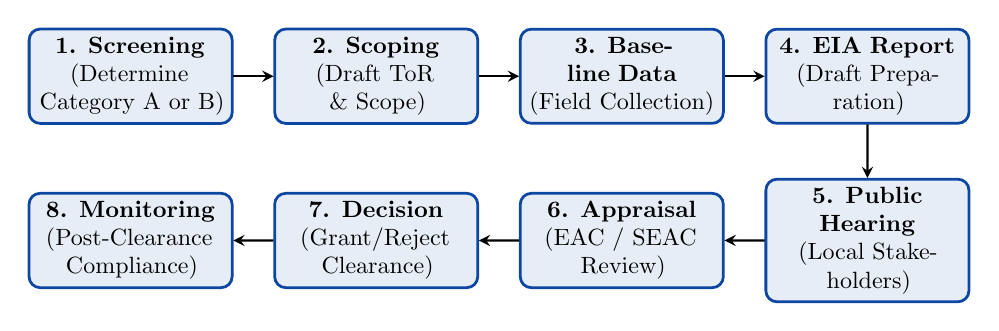
\begin{tikzpicture}[node distance=1.2cm, auto, scale=0.85, transform shape]
  \tikzstyle{block} = [rectangle, draw, fill=primaryblue!10, text width=2.8cm, text centered, rounded corners, minimum height=1cm, line width=1pt, draw=primaryblue]
  \tikzstyle{arrow} = [thick,->,>=stealth]

  \node [block] (step1) {\textbf{1. Screening}\\ (Determine Category A or B)};
  \node [block, right=0.6cm of step1] (step2) {\textbf{2. Scoping}\\ (Draft ToR \& Scope)};
  \node [block, right=0.6cm of step2] (step3) {\textbf{3. Baseline Data}\\ (Field Collection)};
  \node [block, right=0.6cm of step3] (step4) {\textbf{4. EIA Report}\\ (Draft Preparation)};
  
  \node [block, below=0.8cm of step4] (step5) {\textbf{5. Public Hearing}\\ (Local Stakeholders)};
  \node [block, left=0.6cm of step5] (step6) {\textbf{6. Appraisal}\\ (EAC / SEAC Review)};
  \node [block, left=0.6cm of step6] (step7) {\textbf{7. Decision}\\ (Grant/Reject Clearance)};
  \node [block, left=0.6cm of step7] (step8) {\textbf{8. Monitoring}\\ (Post-Clearance Compliance)};

  \draw [arrow] (step1) -- (step2);
  \draw [arrow] (step2) -- (step3);
  \draw [arrow] (step3) -- (step4);
  \draw [arrow] (step4) -- (step5);
  \draw [arrow] (step5) -- (step6);
  \draw [arrow] (step6) -- (step7);
  \draw [arrow] (step7) -- (step8);
\end{tikzpicture}
\end{center}

\subsubsection{National Action Plan on Climate Change (NAPCC)}
Formulated in 2008 comprising 8 Core National Missions:
\begin{enumerate}[leftmargin=*]
  \item National Solar Mission
  \item National Mission for Enhanced Energy Efficiency (NMEEE)
  \item National Mission on Sustainable Habitat
  \item National Water Mission
  \item National Mission for Sustaining the Himalayan Ecosystem
  \item National Mission for a ``Green India'' (Afforestation)
  \item National Mission for Sustainable Agriculture
  \item National Mission on Strategic Knowledge for Climate Change
\end{enumerate}

\subsection{Resource Potentials and Resource Regions}

\begin{defbox}[Resource Region]
A Resource Region is a spatial unit of the earth's surface that exhibits structural homogeneity in its natural resource potential, environmental conditions, and socio-economic development challenges, serving as an ideal geographic unit for regional planning.
\end{defbox}

\subsubsection{1. Planning Commission's 15 Agro-Climatic Regions}
Formulated in 1988 for regional agricultural planning based on rainfall, temperature, soil type, water resources, and cropping systems:
\begin{enumerate}[leftmargin=*]
  \item Western Himalayan Region (J\&K, Himachal, Uttarakhand; temperate fruits, maize).
  \item Eastern Himalayan Region (NE states, N. Bengal; high rainfall, rice, tea, shifting cultivation).
  \item Lower Gangetic Plains Region (W. Bengal; high rainfall, alluvial soil, rice, jute).
  \item Middle Gangetic Plains Region (E. UP, Bihar; high population, rice, wheat, sugarcane).
  \item Upper Gangetic Plains Region (W. UP; canal irrigation, intensive wheat, sugarcane).
  \item Trans-Gangetic Plains Region (Punjab, Haryana, Delhi; tube-well irrigation, high mechanization, wheat, rice).
  \item Eastern Plateau and Hills Region (Chota Nagpur, Odisha, Chhattisgarh; rainfed, rice, coarse grains, rich minerals).
  \item Central Plateau and Hills Region (MP, Rajasthan; dryland farming, pulses, oilseeds).
  \item Western Plateau and Hills Region (Maharashtra, Malwa; black soil, cotton, jowar, sugarcane).
  \item Southern Plateau and Hills Region (Telangana, Rayalaseema, Interior TN, N. Karnataka; dryland, millets).
  \item East Coast Plains and Hills Region (Coromandel \& Andhra coasts; fertile deltas, wet paddy).
  \item West Coast Plains and Ghats Region (Malabar \& Konkan coasts; high rainfall, coconut, spices, rice).
  \item Gujarat Plains and Hills Region (Gujarat; black/alluvial soils, cotton, groundnut).
  \item Western Dry Region (Thar desert, W. Rajasthan; extreme aridity, bajra, livestock).
  \item The Islands Region (Andaman, Nicobar, Lakshadweep; equatorial climate, coconut, plantation crops).
\end{enumerate}

\subsubsection{2. P. Sen Gupta's Resource Regionalization Scheme}
Miss P. Sen Gupta (1968) divided India into a hierarchical framework of resource regions based on physical resource base, population capacity, and degree of economic development:
\begin{itemize}[leftmargin=*]
  \item \textbf{6 Macro Resource Regions}:
  \begin{enumerate}
    \item \textit{North-Eastern Macro Region}: Rich forest, bio-diversity, hydro potential; tea, oil; hilly relief obstacle.
    \item \textit{Eastern Macro Region}: Chota Nagpur & Gangetic delta; mineral heartland (coal, iron, bauxite), heavy industry.
    \item \textit{Central Macro Region}: Vindhya-Satpura plateaus; timber, pulses, oilseeds, moderate mineral wealth.
    \item \textit{Southern Macro Region}: Deccan plateau & coastal plains; black soil, cotton, cash crops, IT hubs.
    \item \textit{Western Macro Region}: Arid/semi-arid plains; cotton, oilseeds, solar/wind energy, commercial trade.
    \item \textit{Northern Macro Region}: Indo-Gangetic alluvial plains & Himalayas; food bowl of India (wheat/rice), river water.
  \end{enumerate}
  \item \textbf{42 Meso Resource Regions}: Sub-divisions based on secondary resource characteristics.
  \item \textbf{129 Micro Resource Regions}: Local planning units.
\end{itemize}

\newpage
% ==========================================
% UNIT IV: RESOURCE PERSPECTIVE & CASE STUDIES
% ==========================================
\section{Unit IV: Resource Perspective --- Regional Planning, Models \& Case Studies}

\subsection{Agriculture Regions}

\subsubsection{D. Whittlesey's World Agricultural Regionalization (1936)}
Derwent Whittlesey delineated world agriculture into 13 major regions based on 5 functional criteria:
\begin{enumerate}[leftmargin=*]
  \item \textbf{Nomadic Herding}: Extensivity in arid/semi-arid zones (e.g., Sahara, Central Asia).
  \item \textbf{Livestock Ranching}: Commercial grazing in temperate grasslands (e.g., Pampas, US West).
  \item \textbf{Shifting Cultivation}: Slash-and-burn in tropical rainforests (e.g., Amazon, Congo, NE India).
  \item \textbf{Rudimentary Sedentary Tillage}: Tropical subsistence agriculture without land rotation.
  \item \textbf{Intensive Subsistence with Paddy Dominance}: High labor intensity in monsoon Asia (India, SE China).
  \item \textbf{Intensive Subsistence without Paddy}: Dryland crops (wheat, millets) in drier monsoon Asia.
  \item \textbf{Commercial Plantation}: Tropical export cash cropping (tea, coffee, rubber, sugarcane).
  \item \textbf{Mediterranean Agriculture}: Specialized citrus, vine, olive, and winter grain production.
  \item \textbf{Commercial Grain Farming}: Extensive mechanized wheat production (e.g., US Prairies, Ukrainian Steppes).
  \item \textbf{Commercial Livestock and Crop Farming (Mixed Farming)}: Integrated crop-feed-livestock systems (Western Europe).
  \item \textbf{Commercial Dairy Farming}: Specialized milk production (e.g., Denmark, New Zealand, US Great Lakes).
  \item \textbf{Specialized Horticulture}: Intensive fruit and flower farming.
  \item \textbf{Commercial Market Gardening (Truck Farming)}: Perishable vegetable farming surrounding urban centers.
\end{enumerate}

\subsubsection{Agricultural Regionalization of India}
\begin{itemize}[leftmargin=*]
  \item \textbf{Jasbir Singh's Crop Combination Method (1974)}: Applied **Wilford Weaver's Minimum Deviation Method** ($\sigma^2 = \frac{\sum (d^2)}{n}$) to determine actual crop combinations in India (e.g., Mono-crop Rice, Rice-Wheat combination, Cotton-Jowar combination).
  \item \textbf{ICAR Classification}: India categorized into 5 major agricultural regions: Rice Region, Wheat Region, Millet Region, Temperate Himalayan Region, and Plantation Crops Region.
\end{itemize}

\subsection{Population-Resource Regions}

\begin{modelbox}[Ackerman's Population-Resource Regionalization Model]
Formulated by \textbf{Edward A. Ackerman} (1959). Classified the world into 5 distinct population-resource region types based on three spatial variables: Population density ($P$), Resource availability ($R$), and Technological state ($T$).
\end{modelbox}

\begin{enumerate}[leftmargin=*]
  \item \textbf{Technology-Source / High-Technology Regions (United States Type)}:
  \begin{itemize}
    \item \textit{Features}: Low to medium population density, vast rich natural resources, exceptionally high technology level ($T$). Rapid capital growth and high standard of living.
    \item \textit{Examples}: USA, Canada, Australia, New Zealand.
  \end{itemize}

  \item \textbf{European Type}:
  \begin{itemize}
    \item \textit{Features}: High population density relative to land area, limited natural resources, but extremely high technology ($T$) and highly skilled human capital enabling global resource import and processing.
    \item \textit{Examples}: UK, Western Europe, Japan.
  \end{itemize}

  \item \textbf{Technology-Deficient / Low-Technology Regions (Egyptian Type)}:
  \begin{itemize}
    \item \textit{Features}: Intense population pressure ($P$), severely limited land resources ($R$), and deficient/developing technology ($T$). Chronic unemployment and food strain.
    \item \textit{Examples}: Egypt, India, Pakistan, Bangladesh.
  \end{itemize}

  \item \textbf{Brazilian Type}:
  \begin{itemize}
    \item \textit{Features}: Low population density ($P$), immense unexploited natural resources ($R$), but deficient technology ($T$) preventing full resource appraisal.
    \item \textit{Examples}: Brazil, interior South America, DRC / Central Africa.
  \end{itemize}

  \item \textbf{Arctic-Desert Type}:
  \begin{itemize}
    \item \textit{Features}: Extreme harsh environment, very sparse population, low technology utilization.
    \item \textit{Examples}: Antarctica, core Sahara desert, high Arctic tundra.
  \end{itemize}

  \item \textbf{Position of India}: India is placed under the **Egyptian Type** due to high population pressure on land. However, India's rapid technological advancement (ISRO, IT sector, green energy) is actively pushing it toward the **European Type** trajectory.
\end{enumerate}

\newpage
\subsection{Resource Planning Units and Development Strategies: Regional Case Studies}

\begin{casebox}[Case Study 1: Damodar Valley Region (DVR)]
\textbf{Geographical Setting}: Spread across Chota Nagpur Plateau in Jharkhand and West Bengal. The Damodar River was historically known as the ``Sorrow of Bengal'' due to catastrophic annual monsoon floods.
\end{casebox}

\subsubsection{1. Damodar Valley Region (DVR)}
\begin{itemize}[leftmargin=*]
  \item \textbf{Institutional Establishment (DVC, 1948)}:
  \begin{itemize}
    \item Damodar Valley Corporation (DVC) was enacted on July 7, 1948, as India's first multi-purpose river valley project.
    \item Explicitly modeled after America's **Tennessee Valley Authority (TVA)**.
  \end{itemize}

  \item \textbf{Multi-Purpose Planning Objectives}:
  \begin{enumerate}
    \item Flood control in the lower Gangetic delta of West Bengal.
    \item Irrigation expansion across $5.5$ lakh hectares via canal networks.
    \item Hydro-electric and thermal power generation.
    \item Soil conservation, afforestation, and navigation.
  \end{enumerate}

  \item \textbf{Major Infrastructure Built}:
  \begin{itemize}
    \item \textit{Dams}: Built at **Tilaiya** and **Maithon** (Barakar River), **Panchet** (Damodar River), and **Konar** (Konar River).
    \item \textit{Barrage}: **Durgapur Barrage** controlling 2,495 km of irrigation and navigation canals.
    \item \textit{Thermal Power Stations}: Bokaro, Durgapur, Chandrapura, Mejia.
  \end{itemize}

  \item \textbf{Resource Base \& Industrial Growth}:
  \begin{itemize}
    \item The DVR is India's premier mineral heartland: Jharia and Raniganj coalfields, Kodarma mica belt, Singhbhum copper and iron ore.
    \item Created the **Heavy Industrial Corridor of Eastern India**: Bokaro Steel Plant, Durgapur Steel Plant, IISCO Burnpur, Chittaranjan Locomotive Works, Sindri Fertilizer Plant.
  \end{itemize}

  \item \textbf{Critical Evaluation \& Planning Challenges}:
  \begin{itemize}
    \item \textit{Achievements}: Tamed destructive floods, electrified eastern India, built heavy manufacturing base.
    \item \textit{Drawbacks}: Heavy siltation reduced dam storage capacities; open-cast mining caused extensive land degradation; severe thermal power fly-ash pollution; displacement of local tribal populations without adequate rehabilitation.
  \end{itemize}
\end{itemize}

\begin{casebox}[Case Study 2: National Capital Region (NCR)]
\textbf{Geographical Setting}: Encompasses National Capital Territory (NCT) of Delhi and 24 surrounding districts across Haryana (Gurugram, Faridabad), Uttar Pradesh (Noida, Greater Noida, Ghaziabad), and Rajasthan (Alwar, Bharatpur), covering $\sim 55,083 \text{ km}^2$.
\end{casebox}

\subsubsection{2. National Capital Region (NCR)}
\begin{itemize}[leftmargin=*]
  \item \textbf{Planning Mandate (NCR Planning Board Act, 1985)}:
  \begin{itemize}
    \item Designed to prevent chaotic urban sprawl in Delhi by creating a balanced regional growth unit.
  \end{itemize}

  \item \textbf{Core Planning Strategies}:
  \begin{enumerate}
    \item \textbf{De-congestion of Core Delhi}: Diverting population influx away from NCT Delhi to surrounding ring towns.
    \item \textbf{Counter-Magnet Towns Strategy}: Developing selected urban nodes outside NCR (e.g., Hissar, Bareilly, Gwalior, Kota, Ambala, Patiala) as self-contained economic hubs to absorb potential migrants before they reach Delhi.
    \item \textbf{Specialized Economic Satellite Clusters}:
    \begin{itemize}
      \item \textit{Gurugram}: Cyber City, IT, financial, and automotive hub.
      \item \textit{Noida / Greater Noida}: Electronics manufacturing, IT, educational hubs.
      \item \textit{Ghaziabad \& Faridabad}: Heavy industrial and manufacturing hubs.
    \end{itemize}
    \item \textbf{Transit-Oriented Transport Infrastructure}:
    \begin{itemize}
      \item Peripheral Expressways: Eastern Peripheral Expressway (EPE) and Western Peripheral Expressway (WPE / KMP) bypassing heavy freight traffic away from Delhi.
      \item **RRTS (Regional Rapid Transit System)**: High-speed Namo Bharat rail corridors connecting Delhi to Meerut, Alwar, and Panipat.
    \end{itemize}
  \end{enumerate}

  \item \textbf{Environmental and Urban Challenges}:
  \begin{itemize}
    \item Severe winter air pollution ($\text{PM}_{2.5} > 400\,\mu\text{g/m}^3$) due to stubble burning, industrial emissions, and vehicular congestion.
    \item Depletion of groundwater tables; encroaching construction on the Aravali Ridge ecosystem; Yamuna river pollution.
  \end{itemize}
\end{itemize}

\begin{casebox}[Case Study 3: Ken-Betwa River Interlinking Project]
\textbf{Geographical Setting}: Spread across Bundelkhand region of Madhya Pradesh and Uttar Pradesh. First major river interlinking project executed under National Perspective Plan.
\end{casebox}

\subsubsection{3. Ken-Betwa River Interlinking Project}
\begin{itemize}[leftmargin=*]
  \item \textbf{Core Objective}: Transfer surplus water from Ken river basin in MP to water-deficit Betwa river basin in UP/MP to irrigate drought-prone Bundelkhand (districts of Panna, Tikamgarh, Chhatarpur, Banda, Mahoba).
  \item \textbf{Infrastructure Components}: Construction of **Daudhan Dam**, $221\text{ km}$ link canal, two tunnels, and hydro-power units.
  \item \textbf{Ecological Debates}: Inundation of $\sim 6,000$ hectares of forest land within **Panna Tiger Reserve**, raising biodiversity concerns vs. drinking water relief for 62 lakh people.
\end{itemize}

\newpage
% ==========================================
% UNIT V: EXAM REVISION & MODEL ANSWERS
% ==========================================
\section{Unit V: Exam Quick Revision \& Model Answer Outlines}

\begin{exambox}[Model Answer Outline 1: Methods of Resource Appraisal]
\textbf{Exam Question}: \textit{``Critically evaluate the methods and techniques of Resource Appraisal. How have Remote Sensing and GIS revolutionized modern resource planning?''} (15 Marks)
\end{exambox}

\subsubsection{Structure for a 15-Mark Model Answer}
\begin{enumerate}[leftmargin=*]
  \item \textbf{Introduction (2 Marks)}: Define Resource Appraisal. Mention its role in identifying physical, economic, and ecological feasibility of resources.
  \item \textbf{Survey \& Spatial Techniques (4 Marks)}:
  \begin{itemize}
    \item Ground surveys vs. **Remote Sensing (RS)**.
    \item Explain NDVI ($\frac{\text{NIR}-\text{Red}}{\text{NIR}+\text{Red}}$) for vegetation health.
    \item Explain **GIS** spatial overlay, DEM, and buffer analysis.
  \end{itemize}
  \item \textbf{Economic Appraisal (3 Marks)}: Explain Cost-Benefit Analysis (CBA), Net Present Value ($\text{NPV} = \sum \frac{B_t-C_t}{(1+r)^t}$), and Internal Rate of Return (IRR).
  \item \textbf{Ecological Appraisal (3 Marks)}: Explain Environmental Impact Assessment (EIA), Ecological Footprint, and Carrying Capacity.
  \item \textbf{Critique \& Conclusion (3 Marks)}: Discuss technological limitations (cloud cover in RS, GIS data errors, high cost) and conclude with the necessity of integrating spatial tech with ground truth validation.
\end{enumerate}

\begin{exambox}[Model Answer Outline 2: Damodar Valley Region Case Study]
\textbf{Exam Question}: \textit{``Discuss the Damodar Valley Corporation (DVC) as a pioneer model of multi-purpose regional resource planning in India. Examine its achievements and environmental drawbacks.''} (15 Marks)
\end{exambox}

\subsubsection{Structure for a 15-Mark Model Answer}
\begin{enumerate}[leftmargin=*]
  \item \textbf{Introduction (2 Marks)}: Location of Damodar basin (Jharkhand/West Bengal). Historical title: ``Sorrow of Bengal''. Establishment of DVC in 1948 modeled on US TVA.
  \item \textbf{Planning Objectives (3 Marks)}: Flood control, canal irrigation, hydro and thermal power generation, soil conservation, industrialization.
  \item \textbf{Physical Infrastructure \& Achievements (5 Marks)}:
  \begin{itemize}
    \item Dams (Tilaiya, Maithon, Panchet, Konar) and Durgapur Barrage.
    \item Creation of Eastern Industrial Belt: Bokaro, Durgapur, Jamshedpur, Raniganj coalfields.
  \end{itemize}
  \item \textbf{Environmental Drawbacks \& Challenges (4 Marks)}: Reservoir siltation, land degradation from open-cast coal mining, thermal power fly ash, tribal displacement.
  \item \textbf{Conclusion (1 Mark)}: Summary of lessons learned for modern river basin planning (e.g., Ken-Betwa link).
\end{enumerate}

\begin{exambox}[Model Answer Outline 3: Seven Approaches in Resource Management]
\textbf{Exam Question}: \textit{``Elaborate on the major approaches in Resource Geography. Contrast the Ecological Approach with the Economic and Institutional Approaches.''} (15 Marks)
\end{exambox}

\subsubsection{Structure for a 15-Mark Model Answer}
\begin{enumerate}[leftmargin=*]
  \item \textbf{Introduction (2 Marks)}: Define resource management approaches as interdisciplinary frameworks for resource planning.
  \item \textbf{Ecological Approach (4 Marks)}: Focus on ecosystem services, Odum's energy flow, natural carrying capacity, physical science basis.
  \item \textbf{Economic Approach (3 Marks)}: Market mechanisms, allocative efficiency, cost-benefit analysis, Hotelling extraction rate.
  \item \textbf{Institutional \& Community Approaches (4 Marks)}: Property rights, legal frameworks, Joint Forest Management (JFM), traditional ecological knowledge (TEK).
  \item \textbf{Synthesis \& Conclusion (2 Marks)}: Emphasize the necessity of an **Integrated Approach** combining ecological, economic, and institutional dimensions.
\end{enumerate}

\begin{exambox}[Model Answer Outline 4: Sustainable Resource Development]
\textbf{Exam Question}: \textit{``Examine the concept, historical evolution, and core dimensions of Sustainable Development. Discuss the significance of Agenda 21 and Agenda 2030 (SDGs).''} (15 Marks)
\end{exambox}

\subsubsection{Structure for a 15-Mark Model Answer}
\begin{enumerate}[leftmargin=*]
  \item \textbf{Introduction \& Definition (2 Marks)}: Brundtland Commission Report (1987) definition (\textit{``Meeting present needs without compromising future generations...''}).
  \item \textbf{Historical Evolution (3 Marks)}: Club of Rome (*Limits to Growth* 1972) $\rightarrow$ Stockholm 1972 $\rightarrow$ Brundtland 1987 $\rightarrow$ Rio Earth Summit 1992 $\rightarrow$ UN SDGs 2015.
  \item \textbf{Dimensions of Sustainable Development (4 Marks)}: Ecological, Economic, Social/Equity, and Governance dimensions. Contrast Weak vs. Strong Sustainability.
  \item \textbf{Agenda 21 \& Agenda 2030 SDGs (5 Marks)}: Detail 4 sections of Agenda 21 and key SDGs (SDG 6 Water, SDG 7 Energy, SDG 13 Climate Action, SDG 15 Life on Land).
  \item \textbf{Conclusion (1 Mark)}: Call for global cooperative action to achieve planetary boundaries.
\end{enumerate}

\begin{exambox}[Model Answer Outline 5: Soil Conservation & Land Capability]
\textbf{Exam Question}: \textit{``Discuss soil degradation concerns in India. Explain the Land Capability Classification (LCC) framework and its utility in watershed management.''} (15 Marks)
\end{exambox}

\subsubsection{Structure for a 15-Mark Model Answer}
\begin{enumerate}[leftmargin=*]
  \item \textbf{Introduction (2 Marks)}: Extent of soil degradation in India ($>30\%$ land degraded).
  \item \textbf{Soil Degradation Types (4 Marks)}: Sheet/rill/gully erosion (Chambal ravines), waterlogging, salinization (\textit{Reh/Usar}).
  \item \textbf{Land Capability Classification (LCC) (5 Marks)}: Detail Classes I--IV (arable) and Classes V--VIII (non-arable/forestry/preservation).
  \item \textbf{Watershed Management Application (3 Marks)}: Integrating LCC into contour bunding, check dams, and agro-forestry.
  \item \textbf{Conclusion (1 Mark)}: Sustainable soil health management for national food security.
\end{enumerate}

\end{document}
